\subsection{Segmentação}

Existem três principais nichos sendo eles: segmentação semântica que é a classifiicação por pixel, a segmentação de instância que atribui um id para cada objeto encontrado de uma classe, e a segmentação panóptica que junta as duas anteriores para criar uma imagem semelhante a saída de segmentação semântica porém separando objetos de mesma classe sendo essa a mais recente e completa, a diferença entre esses três tipos está ilustrado na \cref{fig:segentacoes} \cite{dp_semantic_segmantation, lapix}. 

\begin{figure}[H]
	\caption{Tipos de segmentação em redes neurais convolucionais}
	\centering % para centralizarmos a figura
	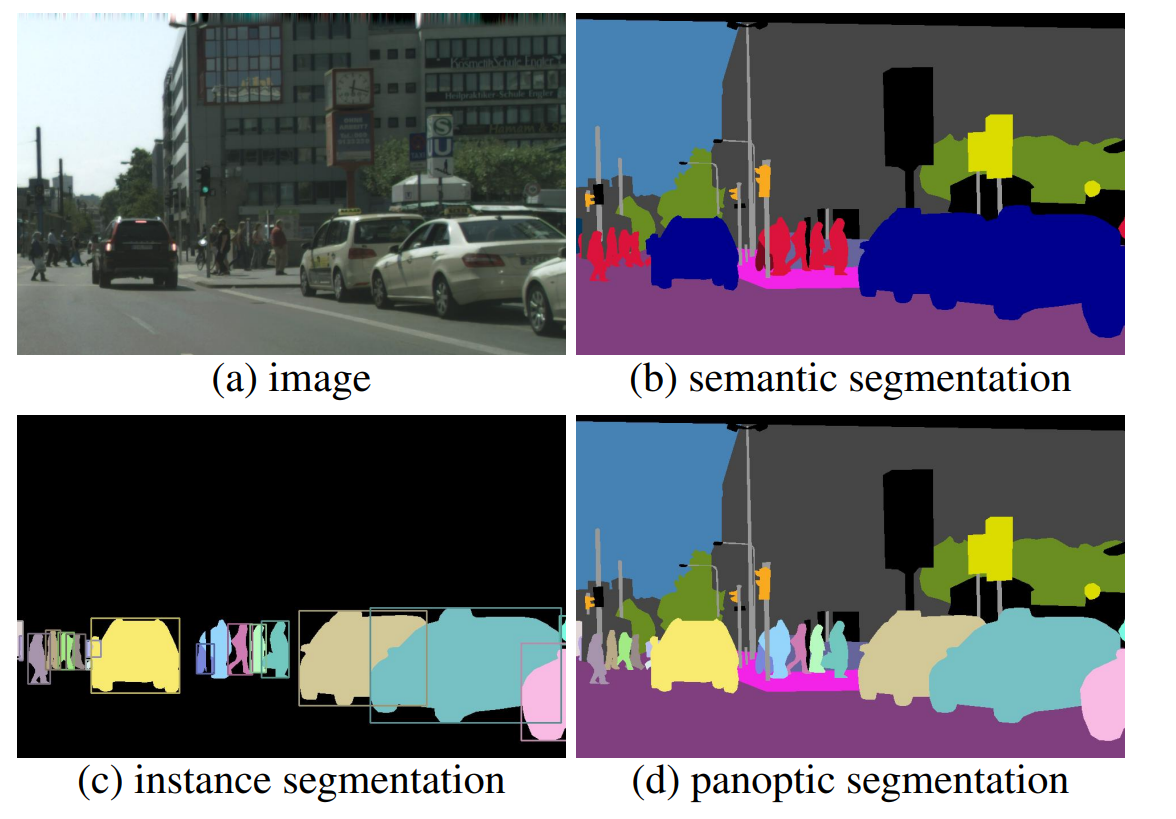
\includegraphics[width=10cm]{figures/segmantations.png} % leia abaixo
	\legend{Fonte: \citeonline{kirillov2019panoptic}}
	\label{fig:segentacoes}
\end{figure}

\subsubsection*{Segmentação semântica}

O estudo de segmentação semântica dentro da área de redes neurais convolucionais começou a ter resultados satisfatórios a partir de redes totalmente convolucionais, um modelo que descarta a camada totalmente conectada pois a saída deverá ser uma imagem e não uma classificação — isso a torna mais rápida para treinar do que as redes neurais convolucionais —, logo usa camadas deconvolucionais para transformar a matriz de características em uma imagem de qualquer dimensão na saída. A RTC criou a arquitetura chamada de salto (ou conexões) que serve para evitar perdas em camadas de agrupamento criando conexões entre camadas não consecutivas — geralmente entre camadas convolucionais e deconvolucionais — como apresentado na \cref{fig:rtc}, a arquitetura de salto evolui para arquitetura codificador-decodificador, o objetivo da RTC é segmentar imagens classificando pixels.
\begin{figure}[H]
	\caption{Exeplo de arquitetura de rede totalmente convolucional}
	\centering % para centralizarmos a figura
	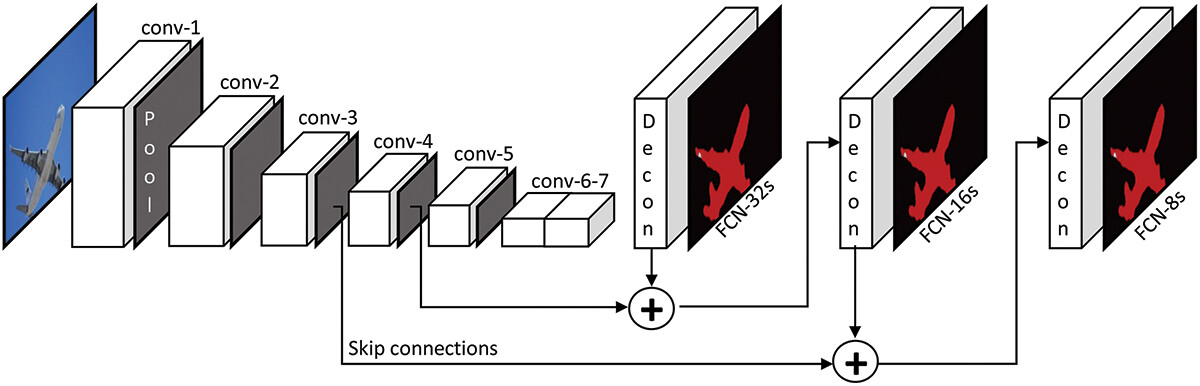
\includegraphics[width=10cm]{figures/redes_totalmente_convolucionais.jpeg} % leia abaixo
	\legend{Fonte: \citeonline{dp_semantic_segmantation}}
	\label{fig:rtc}
\end{figure}

% A arquitetura codificador-decodificador — ou Encoder-Decoder — , que separa em dois passos: o primeiro para convergir no mapa de características — o modelo de redes totalmente convolucionais — e o segundo para reverter em uma imagem usando camadas deconvolucionais e de desagrupamento, como por exemplo a arquitetura UNet que foi a primeira a implementar o padrão Encoder-Decoder. Na \cref{} podemos observar que tem formato da letra U, sendo a descida a parte de Encoder e subida Decoder \cite{dp_semantic_segmantation, lapix}.

\begin{figure}[H]
	\caption{Tipos de segmentação em redes neurais convolucionais}
	\centering % para centralizarmos a figura
	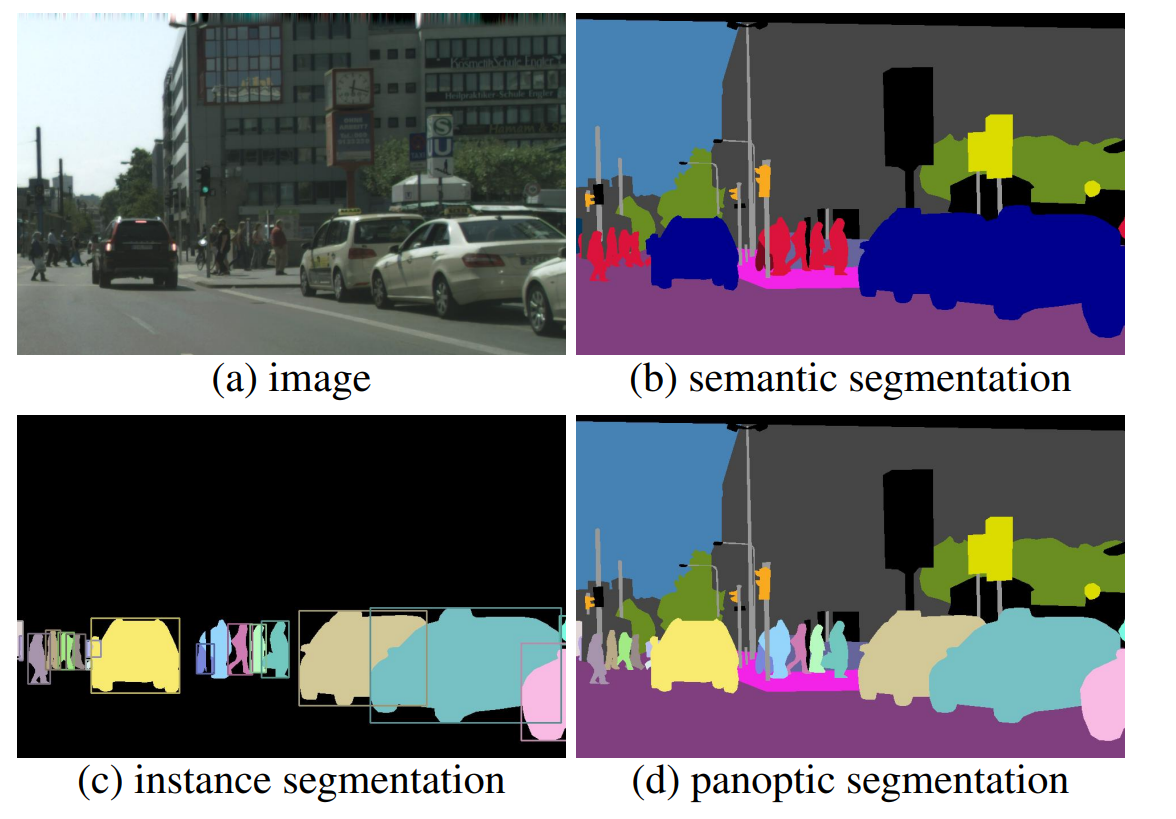
\includegraphics[width=10cm]{figures/segmantations.png} % leia abaixo
	\legend{Fonte: \citeonline{kirillov2019panoptic}}
	\label{fig:segentacoes}
\end{figure}


\subsubsection*{Segmentação de instância}


\subsubsection*{Segmentação panóptica}



\subsubsection*{Modelo escolhido}

% Com base na imagem acima percebemos que segmentação panóptica é a melhor opção para nossa aplicação além do fato de ser a mais nova. Portanto abordaremos métricas para escolher um modelo dentro dessa área de estudo.

% Variações de arquiteturas